\documentclass[../../main/main.tex]{subfiles}
\graphicspath{{./figures/}}

\dominitoc
\faketableofcontents

% \renewcommand{\mtcSfont}{\small\bfseries}
% \renewcommand{\mtcSSfont}{\footnotesize}
\mtcsettitle{minitoc}{}
\mtcsetrules{*}{off}

\makeatletter
\renewcommand{\@chapapp}{Thermodynamique -- chapitre}
\makeatother

% \toggletrue{student}
% \toggletrue{corrige}
% \renewcommand{\mycol}{black}
% \renewcommand{\mycol}{gray}

\hfuzz=5.002pt

\begin{document}
\setcounter{chapter}{1}

\settype{book}
\settype{prof}
\settype{stud}

\chapter{Échanges d'énergie des transformations thermodynamiques}

\vspace*{\fill}

\begin{tcn}*(appl)<ctc>{\iconsomm~Sommaire}
	\vspace{-15pt}
	\minitoc
	\vspace{-25pt}
\end{tcn}

\begin{tcn}*[sidebyside, sidebyside align=top](appl)<ctb>""{\iconhow~Capacités exigibles}
	\begin{itemize}[label=\rcheck]
		\item Définir un système adapté à une problématique donnée.

		\item Exploiter les conditions imposées par le milieu extérieur pour
		      déterminer l'état d'équilibre final.

		\item Évaluer un travail par découpage en travaux élémentaires et sommation
		      sur un chemin donné dans le cas d'une seule variable.
	\end{itemize}
	\tcblower
	\begin{itemize}[label=\rcheck]
		\item Interpréter géométriquement le travail des forces de pression dans un
		      diagramme de \textsc{Watt}.

		\item Distinguer qualitativement les trois types de transferts thermiques~:
		      conduction, convection et rayonnement.

		\item Identifier dans une situation expérimentale le ou les systèmes
		      modélisables par un thermostat.
	\end{itemize}
\end{tcn}

\vspace*{\fill}

\newpage

\vspace*{\fill}
% \begin{boxes}
\begin{tcn}*[sidebyside, fontupper=\small, fontlower=\small](appl)<ctb>{\iconchek~L'essentiel}
	\begin{tcn}*(defi)<ctc>{\icondefi~Définitions}
		\tcblistof[\paragraph*]{defi}{\hspace*{4.8pt}}
	\end{tcn}
	% \begin{tcn}(rapp)<ctc>{\iconrapp~Rappels}
	%   \tcblistof[\paragraph*]{rapp}{\hspace*{4.8pt}}
	% \end{tcn}
	\begin{tcn}*(prop)<ctc>{\iconprop~Propriétés}
		\tcblistof[\paragraph*]{prop}{\hspace*{4.8pt}}
		% \tcblistof[\paragraph*]{loi}{\hspace*{4.8pt}}
		% \tcblistof[\paragraph*]{theo}{\hspace*{4.8pt}}
	\end{tcn}
	% \begin{tcn}*(coro)<ctc>{\iconcoro~Corollaires}
	%   \tcblistof[\paragraph*]{coro}{\hspace*{4.8pt}}
	% \end{tcn}
	\begin{tcn}*(demo)<ctc>{\icondemo~Démonstrations}
		\tcblistof[\paragraph*]{demo}{\hspace*{4.8pt}}
		\tcblistof[\paragraph*]{prev}{\hspace*{4.8pt}}
	\end{tcn}
	% \begin{tcn}*(inte)<ctc>{\iconinte~Interprétations}
	%   \tcblistof[\paragraph*]{inte}{\hspace*{4.8pt}}
	% \end{tcn}
	% \begin{tcn}*(tool)<ctc>{\icontool~Outils}
	% 	\tcblistof[\paragraph*]{tool}{\hspace*{4.8pt}}
	% \end{tcn}
	% \begin{tcn}*(nota)<ctc>{\iconnota~Notations}
	%   \tcblistof[\paragraph*]{nota}{\hspace*{4.8pt}}
	% \end{tcn}
	% \begin{tcn}*(appl)<ctc>{\iconappl~Applications}
	%   \tcblistof[\paragraph*]{appl}{\hspace*{4.8pt}}
	% \end{tcn}
	% \begin{tcn}*(rema)<ctc>{\iconrema~Remarques}
	%   \tcblistof[\paragraph*]{rema}{\hspace*{4.8pt}}
	% \end{tcn}
	% \begin{tcn}*(exem)<ctc>{\iconexem~Exemples}
	%   \tcblistof[\paragraph*]{exem}{\hspace*{4.8pt}}
	% \end{tcn}
	% \begin{tcn}*(ror)<ctc>{\iconhart~Points importants}
	%   \tcblistof[\paragraph*]{ror}{\hspace*{4.8pt}}
	% \end{tcn}
	% \begin{tcn}*(impo)<ctc>{\iconimpo~Erreurs communes}
	%   \tcblistof[\paragraph*]{impo}{\hspace*{4.8pt}}
	% \end{tcn}
	\tcblower
	% \begin{tcn}*(defi)<ctc>{\icondefi~Définitions}
	%   \tcblistof[\paragraph*]{defi}{\hspace*{4.8pt}}
	% \end{tcn}
	% \begin{tcn}*(rapp)<ctc>{\iconrapp~Rappels}
	%   \tcblistof[\paragraph*]{rapp}{\hspace*{4.8pt}}
	% \end{tcn}
	% \begin{tcn}*(prop)<ctc>{\iconprop~Propriétés}
	%   \tcblistof[\paragraph*]{prop}{\hspace*{4.8pt}}
	%   \tcblistof[\paragraph*]{loi}{\hspace*{4.8pt}}
	%   \tcblistof[\paragraph*]{theo}{\hspace*{4.8pt}}
	% \end{tcn}
	% \begin{tcn}*(coro)<ctc>{\iconcoro~Corollaires}
	%   \tcblistof[\paragraph*]{coro}{\hspace*{4.8pt}}
	% \end{tcn}
	% \begin{tcn}*(demo)<ctc>{\icondemo~Démonstrations}
	% 	\tcblistof[\paragraph*]{demo}{\hspace*{4.8pt}}
	% 	\tcblistof[\paragraph*]{prev}{\hspace*{4.8pt}}
	% \end{tcn}
	\begin{tcn}*(inte)<ctc>{\iconinte~Interprétations}
		\tcblistof[\paragraph*]{inte}{\hspace*{4.8pt}}
	\end{tcn}
	% \begin{tcn}*(tool)<ctc>{\icontool~Outils}
	%   \tcblistof[\paragraph*]{tool}{\hspace*{4.8pt}}
	% \end{tcn}
	% \begin{tcn}*(nota)<ctc>{\iconnotaNotations}
	%   \tcblistof[\paragraph*]{nota}{\hspace*{4.8pt}}
	% \end{tcn}
	\begin{tcn}*(appl)<ctc>{\iconappl~Applications}
		\tcblistof[\paragraph*]{appl}{\hspace*{4.8pt}}
	\end{tcn}
	% \begin{tcn}*(rema)<ctc>{\iconrema~Remarques}
	%   \tcblistof[\paragraph*]{rema}{\hspace*{4.8pt}}
	% \end{tcn}
	% \begin{tcn}*(exem)<ctc>{\iconexem~Exemples}
	% 	\tcblistof[\paragraph*]{exem}{\hspace*{4.8pt}}
	% \end{tcn}
	\begin{tcn}*(ror)<ctc>{\iconhart~Points importants}
		\tcblistof[\paragraph*]{ror}{\hspace*{4.8pt}}
	\end{tcn}
	\begin{tcn}*(impo)<ctc>{\iconimpo~Erreurs communes}
		\tcblistof[\paragraph*]{impo}{\hspace*{4.8pt}}
	\end{tcn}
\end{tcn}
% \end{boxes}

\vspace*{\fill}
\newpage

\section{Introduction}
\subsection{Nécessité de la thermodynamique}
En mécanique, on pouvait écrire une équation de conservation d'énergie~:
\[
	\Delta{\Ec_m} = W\ind{NC}
\]
Cette approche ne permet cependant pas de décrire des phénomènes pourtant très
simples. Par exemple, en comprimant de l'air dans une seringue on apporte un
travail non nul ($\Ff \times d \neq 0$). Pourtant, entre l'instant initial et
l'instant final le gaz ne gagne ni vitesse ni énergie potentielle~:
\[
	\left\{
	\begin{array}{rcl}
		W_{NC}        & > & 0
		\\
		\Delta{\Ec_m} & = & 0
	\end{array}
	\right.
	\Ra
	\text{impossible~?}
\]
C'est évidemment, comme discuté au chapitre précédent, qu'il ne gagne pas
d'énergie \textbf{macroscopique} mais \textbf{microscopique}, c'est-à-dire de
l'énergie interne.
\bigbreak
L'objectif de ce chapitre est de mettre en place des outils d'analyse et de
descriptions de transformations d'un système thermodynamique et traduire son
évolution en terme d'énergie.

\subsection{Transformations thermodynamiques}
\begin{tcb*}(defi){Transformations thermodynamique}
	Une \textbf{transformation} est un phénomène physique ou chimique qui produit
	la \textbf{variation} d'au moins un \textbf{paramètre d'état} du système.
	L'état de départ est \textit{l'état initial}, celui d'arrivée \textit{l'état
		final}~; ce sont des \textbf{états d'équilibre} du système, c'est-à-dire que
	les paramètres d'état y sont définis, homogènes et constants.
\end{tcb*}

Il sera donc d'autant plus important de spécifier le système d'étude $\Sigma$ en
thermodynamique, puisque l'on traite spécifiquement des échanges entre systèmes.
\textbf{Il sera toujours fermé} pour appliquer les théorèmes de conservation.
\bigbreak
Pour provoquer la transformation d'un système $\Sigma$ il faut imposer à
$\Sigma$ une modification d'une de ses variables d'état ou bien changer les
conditions extérieures. On met ainsi le système \textbf{hors d'équilibre} et il
évolue vers un \textbf{nouvel état d'équilibre}. On connaît toujours l'état
d'équilibre initial, et on s'intéresse à l'état final~; pour ça, on on
appliquera les \textbf{conditions d'équilibre} mécanique et thermique (sauf si
la transformation est trop rapide, voir plus loin), et les
\textbf{caractéristiques de la transformations}.

\subsection{Types de transformations}
\subsubsection{Sur le volume~: transformation isochore}

\begin{tcb*}(defi){Transformation isochore}
	Une transformation est dite \textbf{isochore} quand le \textbf{volume} du
	système est \textbf{constant} au cours de la transformation~:
	\psw{%
		\[
			\boxed{V = \cte \Lra \dd{V} = 0}
		\]
	}%
	\vspace{-15pt}
\end{tcb*}
Avec $V_i$, $V_f$ et $V$ les volumes dans l'état initial, final et courant, si
la transformation est isochore alors $V_i = V = V_f$. Un système fermé dans un
récipient rigide indéformable subit forcément des transformations isochores.

\begin{tcb}[sidebyside](exem)<lftt>{Transformation isochore}
	\psw{Le gaz d'une capsule à chantilly qu'on sort du frigo~: le volume du gaz
		ne varie pas, mais il est hors équilibre thermique initialement. À l'état
		final, $V_f = V_0$ et $T_f = T\ind{ext}$.}
	\tcblower
	\begin{center}
		\sswitch{
			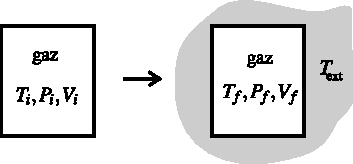
\includegraphics[width=\linewidth, draft=true]{exem_isoV}
		}{
			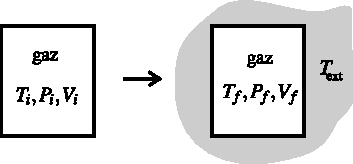
\includegraphics[width=\linewidth]{exem_isoV}
		}
		\vspace{-15pt}
		\captionof{figure}{Schéma}
	\end{center}
\end{tcb}

\subsubsection{Sur la pression~: transformations isobare ou monobare}
\begin{tcb*}[sidebyside](defi){Transformation iso- ou monobare}
	\tcbsubtitle{\fatbox{\textbf{Isobare}}}
	Une transformation est dite \textbf{isobare} quand la \textbf{pression} du
	système est définie et \textbf{constante} au cours de la transformation~:
	\psw{%
		\[
			\boxed{P = \cte \Lra \dd{P} = 0}
		\]
	}%
	\vspace{-15pt}
	\tcblower
	\tcbsubtitle{\fatbox{\textbf{Monobare}}}
	Une transformation \textbf{monobare} est une transformation au cours de
	laquelle la \textbf{pression extérieure} sur les parois mobiles est
	\textbf{constante}~: \psw{%
		\[
			\boxed{P\ind{ext} = \cte}
		\]
	}%
	\vspace{-15pt}
\end{tcb*}

Avec $P_i$, $P_f$ et $P$ les pressions dans l'état initial, final et courant, si
la transformation est isobare alors $P_i = P = P_f$. En pratique une
transformation isobare est une transformation assez lente, dans laquelle on
impose de l'extérieur sa pression au système.

\begin{tcb}[cnt](coro){Isobare et monobare}
	Une transformation \textbf{isobare} est forcément \textbf{monobare} si le
	système a une \textbf{paroi mobile}.
\end{tcb}

\begin{tcb}[sidebyside](exem){Transformation isobare}
	\psw{%
		Gaz dans un récipient avec un piston subissant une force constante, d'état
		initial $T_i, P_i, V_i$. On le place dans un milieu extérieur à la
		température $T\ind{ext}$. À l'état d'équilibre final, $P_f = P = P_i$ par
		construction et $T_f = T\ind{ext}$ puisque c'est un équilibre.
	}%
	\tcblower
	\begin{center}
		\sswitch{
			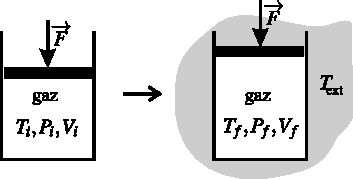
\includegraphics[width=\linewidth, draft=true]{exem_isoP}
		}{
			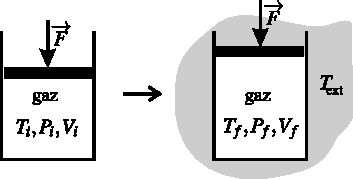
\includegraphics[width=\linewidth]{exem_isoP}
		}
		\vspace{-15pt}
		\captionof{figure}{Schéma}
	\end{center}
\end{tcb}

\subsubsection{Sur la température~: transformations isotherme ou monotherme}
\begin{tcb*}[sidebyside](defi){Transformation iso- ou monotherme}
	\tcbsubtitle{\fatbox{\textbf{Isotherme}}}
	Une transformation est dite \textbf{isotherme} quand la \textbf{température} du
	système est définie et \textbf{constante} au cours de la transformation~:
	\psw{%
		\[
			\boxed{T = \cte \Lra \dd{T} = 0}
		\]
	}%
	\vspace{-15pt}
	\tcblower
	\tcbsubtitle{\fatbox{\textbf{Monotherme}}}
	Une transformation \textbf{monotherme} est une transformation au cours de
	laquelle la \textbf{température extérieure} lors d'un transfert thermique est
	\textbf{constante}~: \psw{%
		\[
			\boxed{T\ind{ext} = \cte}
		\]
	}%
	\vspace{-15pt}
\end{tcb*}

Avec $T_i$, $T_f$ et $T$ les températures dans l'état initial, final et courant,
si la transformation est isotherme alors $T_i = T = T_f$. Ces conditions sont
très contraignantes et difficilement réalisables en pratique. La transformation
isotherme est une transformation théorique idéale. On reviendra sur ce point
plus tard.

\begin{tcb}[cnt](coro){Isotherme et monotherme}
	Une transformation \textbf{isotherme} est obligatoirement \textbf{monotherme}
	s'il y a un \textbf{transfert thermique}.
\end{tcb}

\begin{tcb}(exem)<lftt>{Transformation monotherme}
	Les deux exemples précédents sont monothermes, mais \textbf{pas isothermes}~:
	au cours de ces transformations, la température du système n'est pas définie
	dans les états intermédiaires qui ne sont pas des états d'équilibre, elle est
	seulement définie dans l'état final.
\end{tcb}

\subsubsection{Sur le transfert thermique~: transformation adiabatique}
Nous définirons dans la partie~\fullref{--}{sec:transtherm} les notions
associées, mais il est crucial d'introduire nettement la différence entre
\textbf{température} et \textbf{transfert thermique}. Notamment, on aura la
définition suivante~:
\begin{tcb}(defi){Transformation adiabatique}
	Une transformation est dite \textbf{adiabatique} s'il n'y a \textbf{pas
		de transfert thermique}~:
	\psw{%
		\[
			\boxed{Q = 0}
		\]
	}%
	\vspace{-15pt}
\end{tcb}
Nous détaillerons plus loin les implications, et l'erreur classique d'une
personne n'ayant pas pris la peine de faire une fiche de vocabulaire, malgré
l'insistance de san professeurx de physique (qui est quand même de bon
conseils~!)…

\subsubsection{Utilisation des informations}

\begin{tcb*}(prop){Équation d'état et transformation}
	On peut déterminer les paramètres d'état de l'état final d'un gaz parfait
	subissant une transformation isochore ou isobare grâce à l'équation d'état du
	gaz parfait~:
	\psw{
		\[
			\frac{P_iV_i}{T_i} = \frac{P_fV_f}{T_f}
			\Ra
			\left\{
			\begin{array}{rclr}
				P_f & = & \DS P_i \frac{T_f}{T_i} & \quad \text{isochore}
				\\
				V_f & = & \DS V_i \frac{T_i}{T_i} & \quad \text{isobare}
			\end{array}
			\right.
		\]
	}
	À partir de l'équilibre thermique par exemple, on détermine la pression
	finale pour une transformation isochore.
\end{tcb*}

\begin{tcb*}(ror){Résumé des transformations}
	Une transformation thermodynamique peut être~:
	\smallbreak
	\begin{isd}[lefthand ratio=.35]
		\begin{itemize}
			\bitem{Isochore}~: \psw{$V = \cte \Lra \dd{V} = 0$}
			\bitem{Isobare}~: \psw{$P = \cte \Lra \dd{P} = 0$}
			\bitem{Monobare}~: \psw{$P\ind{ext} = \cte$}
			\bitem{Isotherme}~: \psw{$T = \cte \Lra \dd{T} = 0$}
			\bitem{Monotherme}~: \psw{$T\ind{ext} = \cte$}
			\bitem{Adiabatique}~: \psw{$Q = 0$}
		\end{itemize}
		\tcblower
		\begin{center}
			\sswitch{
				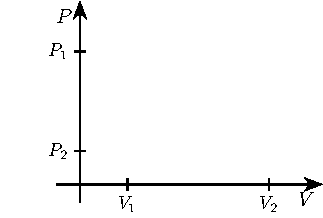
\includegraphics[width=\linewidth]{PV_all-plain}
			}{
				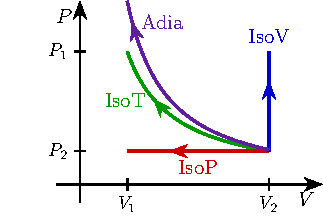
\includegraphics[width=\linewidth]{PV_all}
			}
			\captionof{figure}{Représentations en $(P,V)$}
		\end{center}
	\end{isd}
\end{tcb*}

\subsection{Influence du choix du système}
On aura souvent plusieurs choix de système d'étude. Or, selon le système choisi,
la transformation n'aura pas les mêmes propriétés. Il faudra être
particulièrement vigilant-e à l'établissement du système et de ses propriétés~!

\begin{tcb*}[breakable](appl)<lftt>{Choix d'un système}
	\begin{isd}
		Soit une enceinte indéformable, séparée en deux compartiments par une
		cloison étanche et mobile. Le premier a pour état initial $(T_i,P_i,V_i,n)$,
		le second $(T_i,2P_i,V_i,2n)$. Une cale bloque initialement la cloison
		mobile. On enlève la cale et on place l'enceinte dans un environnement à
		température $T_0$.
		\tcblower
		\begin{center}
			\sswitch{
				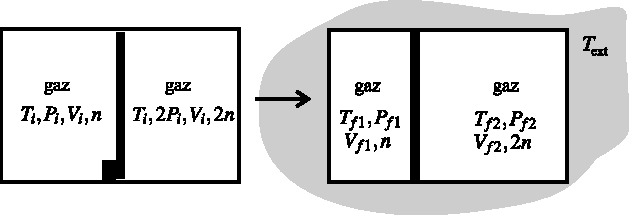
\includegraphics[width=\linewidth, draft=true]{exem_syst}
			}{
				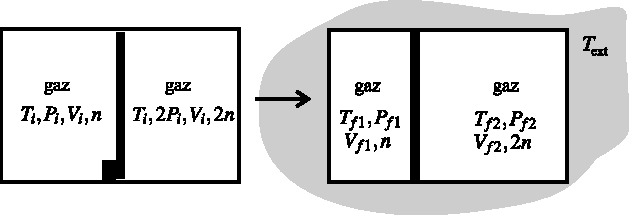
\includegraphics[width=\linewidth]{exem_syst}
			}
			\vspace{-15pt}
			\captionof{figure}{Schéma.}
		\end{center}
	\end{isd}
	\begin{enumerate}
		\item \textbf{Quelles sont les variables d'état des gaz dans l'état
			      d'équilibre final~?}
		\item Qualifier la transformation selon le système étudié.
	\end{enumerate}
	\tcblower
	\begin{enumerate}
		\item \begin{itemize}
			      \bitem{Température}~: \psw{équilibre thermique $\Ra T_{f,1} =
					      T_{f,2} = T_0$~;}
			      \bitem{Pression}~: \psw{équilibre mécanique $\Ra P_{f,1} =
					      P_{f,2}$~;}
			      \bitem{Volume}~:
			      \begin{itemize}
				      \item \psw{Conservation du volume $\Ra 2V_i = V_{f,1} +
						            V_{f,2}$~;}
				      \item \psw{Gaz parfait $\Ra P_{f,1}V_{f,1} = nR T_{f,1} \qet
					            P_{f,2}V_{f,2} = nRT_{f,2} \qdc V_{f,2} = 2V_{f,1}$~;}
				      \item \psw{On combine~: $\DS V_{f,1} = \frac{2}{3}V_i \qet V_{f,2}
						            = \frac{4}{3}V_i$}
			      \end{itemize}
			      D'où
			      \psw{%
				      \[
					      \boxed{P_{f,1} = P_{f,2} = \frac{3}{2}\frac{nRT_0}{V_i}}
				      \]
			      }%
		      \end{itemize}
		\item On a \psw{trois} systèmes~: \psw{$\Sigma_1$, $\Sigma_2$ et $\Sigma =
				      \Sigma_1 + \Sigma_2$.}
		      \begin{itemize}
			      \item \psw{$\Sigma$ est \textbf{isochore} et \textbf{monotherme}~;}
			      \item \psw{$\Sigma_1$ et $\Sigma_2$ n'est \textbf{ni isochore},
				            \textbf{ni monotherme} puisque, sauf indication contraire, il
				            peut y avoir échange thermique à travers la paroi qui les
				            sépare.}
		      \end{itemize}
	\end{enumerate}
\end{tcb*}

\begin{tcb*}(ror){Sens de calcul des variations}
	Au cours d'une transformation, un système échange généralement de l'énergie
	avec l'extérieur. Il faut choisir un sens de comptage.
	\begin{center}
		\bfseries
		Les échanges d'énergie d'un système sont toujours exprimés en valeur
		algébrique~: ils sont positifs lorsque le système choisi reçoit de l'énergie
		et négatifs lorsqu'il en cède.
	\end{center}
\end{tcb*}

\section{Travail des forces de pression}
La force exercée par un fluide sous pression peut être utilisée pour propulser
le piston d'un cylindre, et indirectement le rotor d'un moteur. Le but de cette
partie est de quantifier le travail mécanique fourni lors d'une transformation
thermodynamique.

\subsection{Expression générale}

\begin{tcb*}(prop){Travail des forces de pression}
	Le travail \textbf{reçu} des forces de pression extérieures lors d'une
	variation infinitésimale de volume $\dd{P}$ est~:
	\psw{%
		\[
			\boxed{\delta W_p = -P\ind{ext}\dd{V}}
			\quad \Ra \quad
			W_p = - \int_{V_i}^{V_f}P\ind{ext}\dd{V}
		\]
	}%
\end{tcb*}
\begin{tcb*}[breakable](demo){Travail des forces de pression}
	\begin{isd}[righthand ratio=.4]
		Prenons le cas extrêmement simple d'une seringue de section $S$ avec un piston
		imperméable, pouvant glisser sans frottements et bouchée à son autre
		extrémité. Notons $x$ la longueur de la cavité contenant de l'air.
		\tcblower
		\begin{center}
			\sswitch{
				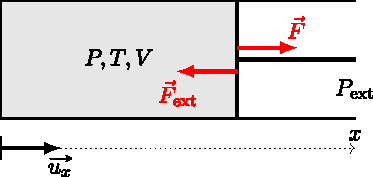
\includegraphics[width=\linewidth, draft=true]{W_demo}
			}{
				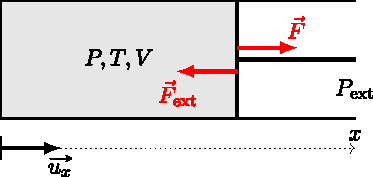
\includegraphics[width=\linewidth]{W_demo}
			}
			% \vspace{-15pt}
			% \captionof{figure}{Schéma.}
		\end{center}
	\end{isd}
	\tcblower
	\begin{itemize}
		\bitem{Système}~: \psw{air de la seringue considéré comme un gaz parfait~;}
		\bitem{Référentiel}~: \psw{laboratoire galiléen~;}
		\bitem{Repère}~: \psw{$(\Or,\ux)$ orienté vers l'\textbf{extérieur}}
		\bitem{Force}~: \psw{$\Ff_p = -P\ind{ext}S \ux$}
		\bitem{Travail}~:
		\leavevmode\vspace*{-15pt}\relax
		\psw{%
			\begin{gather*}
				\delta W_p = \Ff \cdot \dd{\OM} = -P\ind{ext}S \dd{x}
				\\\beforetext{$S \dd{x} = \dd{Sx}$}
				\Lra
				\boxed{\delta W_p = -P\ind{ext} \dd{V}}
				\qed
			\end{gather*}
		}%
		\vspace{-15pt}
	\end{itemize}
\end{tcb*}

\begin{tcb}(rema)<lftt>{Travail des forces de pression}
	\begin{itemize}
		\item Le résultat se généralise pour un système général à pression extérieure
		      \textbf{uniforme}.
		\item Sachant que les énergie sont algébriques, on a~:
		      \begin{itemize}
			      \item $W_p > 0 \Ra$ \psw{système reçoit de l'énergie $\Ra$
				            \textbf{récepteur}}
			      \item $W_p < 0 \Ra$ \psw{système perd de l'énergie $\Ra$
				            \textbf{travail
					            moteur}}%
			      \item Compression~: \psw{$\Lra \dd{V} < 0 \Lra \boxed{\delta W_p > 0}$}
		      \end{itemize}
	\end{itemize}
\end{tcb}

% \subsection{Cas particuliers}
\subsection{Transformations isochore et isobare}

\begin{tcb*}(prop){$W_p$ isochore, monobare}
	Pour les transformations isochore ou monobare, on peut simplifier cette
	expression~:
	\smallbreak
	\begin{isd}[sidebyside align=top]
		\tcbsubtitle{\fatbox{\textbf{Isochore}}}
		\psw{%
			\[
				\boxed{\delta W_p = 0}
				\Lra
				W_p = 0
			\]
		}%
		\vspace{-15pt}
		\tcblower
		\tcbsubtitle{\fatbox{\textbf{Monobare}}}
		\psw{%
			\[
				\boxed{W_p = -P\ind{ext}\Delta{V}}
			\]
		}%
		\vspace{-15pt}
	\end{isd}
\end{tcb*}
\begin{tcb*}[sidebyside, sidebyside align=top, lefthand ratio=.3](demo){$W_p$ isochore, monobare}
	\tcbsubtitle{\fatbox{\textbf{Isochore}}}
	\vspace{-15pt}
	\psw{%
		\begin{gather*}
			\dd{V} = 0 \Ra \delta W_p = 0
			\qed
		\end{gather*}
	}%
	\vspace{-15pt}
	\tcblower
	\tcbsubtitle{\fatbox{\textbf{Monobare}}}
	\vspace{-15pt}
	\psw{%
		\begin{gather*}
			P\ind{ext} = \cte \Ra W_p = -P\ind{ext}\int_{V_i}^{V_f}\dd{V}
			\Lra
			\boxed{W_p = -P\ind{ext}\underbracket[1pt]{\left( V_f - V_i \right)}_{=
			\Delta{V}}}
			\qed
		\end{gather*}
	}%
	\vspace{-15pt}
\end{tcb*}

\begin{tcb}(rema)<lftt>{Autres travaux}
	Celui des forces de pression est \textbf{toujours présent}, mais
	il existe d'autres travaux, par exemple l'effet \textsc{Joule}~:
	\[
		W = \psw{\int u(t)i(t)\dd{t} = RI^2 \Delta{t}}
	\]
\end{tcb}

\subsection{Transformation quasi-statique ou mécaniquement réversible}
\subsubsection{Expression générale}

\begin{tcbraster}[raster equal height=rows, raster columns=5]
	\begin{tcb*}[raster multicolumn=3](defi){Transforma$^\circ$ quasi-statique}
		Une transformation \textbf{quasi-statique} ou \textbf{mécaniquement
			réversible} est une transformation au cours de laquelle l'équilibre mécanique
		est \textbf{réalisé à chaque instant}, soit
		\psw{%
			\[
				\boxed{P = P\ind{ext}}
			\]
		}%
		\vspace{-15pt}
	\end{tcb*}
	\begin{tcb}*[raster multicolumn=2](rema)<rgtt>"lrem"'r'{Condition}
		Il faut que les parties mobiles soient bien plus lentes que la \textbf{vitesse
			du son} dans le gaz, porteur des ondes de pression.
	\end{tcb}
\end{tcbraster}

\begin{tcb*}(impo){Transformation quasi-statique}
	Il faut différencier \textbf{mécaniquement réversible} et \textbf{isobare}~:
	l'équilibre peut être réalisé mais \textbf{la pression peut changer}\ftn{D'où
		l'importance de faire des fiches de vocabulaire.}~!
\end{tcb*}
\begin{tcb*}(prop){$W_p$ quasi-statique}
	Pour une transformation quasi-statique, on remplace la pression extérieure par
	la pression du système~:
	\psw{%
		\[
			\boxed{W_p = - \int_{V_i}^{V_f}P \dd{V}}
		\]
	}%
\end{tcb*}

\vspace{-15pt}
\subsubsection{Interprétation géométrique}

\begin{tcb*}[sidebyside, righthand ratio=.30](inte){$W_p$ quasi-statique en $(P,V)$}
	Puisque la pression est alors bien définie à chaque instant on peut la tracer
	entre les états. Le travail des forces de pression dans le cas mécaniquement
	réversible dans un diagramme de \textsc{Watt} $(P,V)$ est \xul{\psw{égal à
			l'aire sous la courbe}}, et on a~:
	\begin{tasks}[label=\bdmd]
		\task $W > 0 \Lra \psw{\dd{V}<0}$
		\task $W < 0 \Lra \psw{\dd{V}>0}$
	\end{tasks}
	\tcblower
	\begin{center}
		\sswitch{
			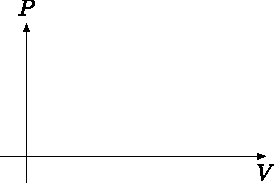
\includegraphics[width=\linewidth]{W_pv-plain.pdf}
		}{
			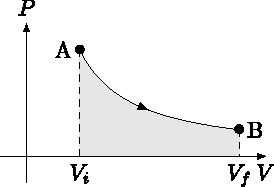
\includegraphics[width=\linewidth]{W_pv.pdf}
		}
		\vspace{-30pt}
		\captionsetup{justification=centering}
		\captionof*{figure}{\\$W_p$ quasi-statique en $(P,V)$}
	\end{center}
\end{tcb*}
\vspace{-15pt}
\begin{tcb}[tabularx={Y|Y|Y}](exem)<lftt>{Quelques travaux en $(P,V)$}
	&&\\
	\sswitch{
		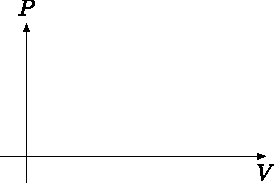
\includegraphics[width=.9\linewidth]{W_pv-plain.pdf}
	}{
		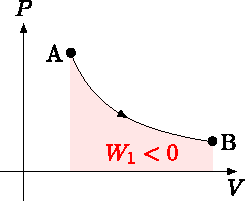
\includegraphics[width=.9\linewidth]{W_pv-exa.pdf}
	}
	\captionsetup{justification=centering}
	\captionof*{figure}{\large Détente~: $W_{p,1}~\psw{<}~0$}
	\vspace*{-15pt}
	&
	\sswitch{
		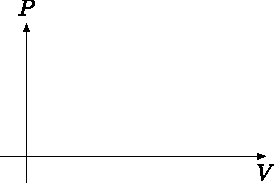
\includegraphics[width=.9\linewidth]{W_pv-plain.pdf}
	}{
		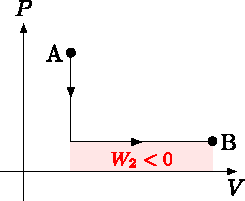
\includegraphics[width=.9\linewidth]{W_pv-exb.pdf}
	}
	\captionsetup{justification=centering}
	\captionof*{figure}{\large Détente~: $W_{p,2}~\psw{<}~W_{p,1}$}
	\vspace*{-15pt}
	&
	\sswitch{
		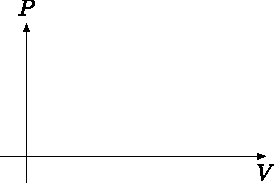
\includegraphics[width=.9\linewidth]{W_pv-plain.pdf}
	}{
		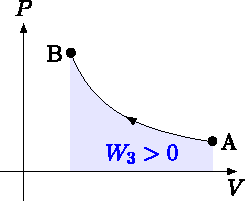
\includegraphics[width=.9\linewidth]{W_pv-exc.pdf}
	}
	\captionsetup{justification=centering}
	\captionof*{figure}{\large Compression~: $W_{p,3}~\psw{>}~0$}
	\vspace*{-15pt}
\end{tcb}

\begin{tcb*}(ror){$W_p$ en $(P,V)$}
	\begin{itemize}
		\item \psw{$\abs{W_p}$ est l'aire sous la courbe~;}
		\item \psw{Le signe de $W_p$ indique une compression ou détente~;}
		\item \psw{Le travail \textbf{dépend du chemin suivi}.}
	\end{itemize}
\end{tcb*}

\begin{tcb*}(appl)<lftt>{$W_p$ quasi-statique et isotherme}
	Déterminer le travail reçu par un gaz parfait lors d'une transformation
	mécaniquement réversible et isotherme, avec $T\ind{ext} = T_0$, en fonction de
	$V_i$ et $V_f$ d'abord, puis en fonction de $P_f$ et $P_i$ en suite. Vérifier
	qu'il est bien négatif si $\dd{V} > 0$.
	\tcblower
	\psw{%
		On est donc à \textbf{l'équilibre thermodynamique} à chaque instant, soit
		\begin{gather*}
			P = P\ind{ext} \qet T = T_0
			\\\Ra
			W_p =
			- \int_{V_i}^{V_f}P \dd{V} =
			-\int_{V_i}^{V_f} \frac{nRT_0}{V}\dd{V}
			\\\Lra
			W_p = -nRT_0 (\ln V_f - \ln V_i)
			\Lra
			\boxed{W_p = nRT_0 \ln (\frac{V_i}{V_f})}
			\\\beforetext{$\frac{V_i}{V_f} = \frac{P_f}{P_i}$ donc}
			\Lra
			\boxed{W_p = -nRT_0 \ln (\frac{P_i}{P_f})}
		\end{gather*}
		Si $\dd{V} > 0$, alors $V_i < V_f \Lra \frac{V_i}{V_f} < 0 \Lra W_p <
			0$~\cmark.
	}%
\end{tcb*}

\subsubsection{Travail reçu sur un cycle}
On s'intéresse à une transformation cyclique du système, au cours de laquelle il
passe d'un état $A$ à un état $B$, puis revient à l'état $A$ par un autre
chemin~: $A \lra B \lra A$.

\begin{tcb*}(prop){$W_p$ sur un cycle $(P,V)$}
	Lors d'une transformation cyclique, le travail total représente \textbf{l'aire
		encapsulée} par la courbe en diagramme $(P,V)$, et on a son signe avec la
	\textbf{règle de la main droite}~:
	\begin{itemize}
		\bitem{Sens direct} $\Ra W_{p,\rm cycle}~\psw{>}~0$ et le cycle est
		\xul{\psw{\textbf{récepteur}}}
		\bitem{Sens horaire} $\Ra W_{p,\rm cycle}~\psw{<}~0$ et le cycle est
		\xul{\psw{\textbf{moteur}}}
	\end{itemize}
\end{tcb*}

\begin{tcb*}[breakable](demo){$W_p$ sur un cycle $(P,V)$}
	On suppose pour fixer les idées que $V_B > V_A$.
	\begin{tasks}[label=\bdmd](2)
		\task \textbf{De $A$ à $B$}~:
		\[
			\psw{W_{p,A\ra B} = -\Ac}
		\]
		avec $\Ac$ l'aire sous la courbe.
		\task \textbf{De $B$ à $A$}~:
		\[
			\psw{W_{p,B\ra A} = \Ac'}
		\]
		avec $\Ac'$ l'aire sous la courbe.
	\end{tasks}
	\begin{itemize}
		\bitem{Sur le cycle}~:
		\psw{%
			le travail \textbf{total} est la \textbf{somme des travaux}
			\[
				W_{p,\rm cycle} = W_{p,A \ra B} + W_{p, B \ra A} = \Ac' - \Ac =
				\Ac\ind{cycle}
			\]
		}%
	\end{itemize}
	\vspace*{-15pt}
	\begin{center}
		\sswitch{
			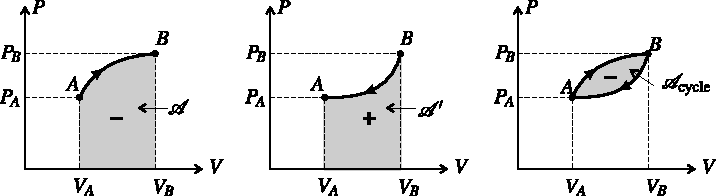
\includegraphics[width=.8\linewidth, draft=true]{W_cycle-demo}
		}{
			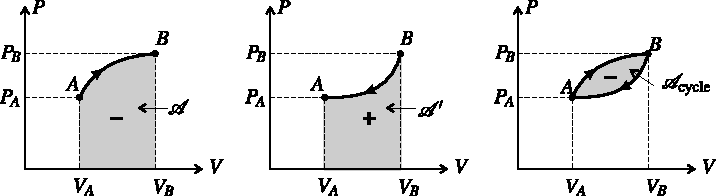
\includegraphics[width=.8\linewidth]{W_cycle-demo}
		}
		\captionof{figure}{Schémas.}
	\end{center}
\end{tcb*}

\begin{tcb}(rema)<lftt>{Travail et paramètre d'état}
	Ces résultats montrent bien que le travail n'est pas la variation d'une
	fonction d'état $X$ entre l'état initial et l'état final puisque~:
	\begin{itemize}
		\item Toute variation $\Delta{X} = X_f - X_i$ d'un \textbf{paramètre d'état}
		      ne \textbf{dépend pas du chemin suivi}, à l'inverse du travail~;
		\item Lors d'un \textbf{cycle}, $\Delta{X}\ind{cycle} = 0$, à l'inverse du
		      travail.
	\end{itemize}
\end{tcb}

\begin{tcb*}[breakable](appl)<lftt>{Cycle de \textsc{Lenoir}}
	\begin{isd}[righthand ratio=.40]
		On fait subir à $\SI{1}{mol}$ de gaz parfait le cycle suivant~:
		\begin{enumerate}[label=\clalphi]
			\item $P_A = \SI{2e5}{Pa}$ et $V_A = \SI{14}{L}$~;
			\item Chauffage isochore, $P_B = 2P_A = \SI{4e5}{Pa}$~;
			\item Détente isotherme quasi-statique, $V_C = 2V_B = \SI{28}{L}$~;
			      \item[cl](A) Refroidissement isobare, on retourne à l'état initial.
		\end{enumerate}
		\tcblower
		\begin{center}
			\sswitch{
				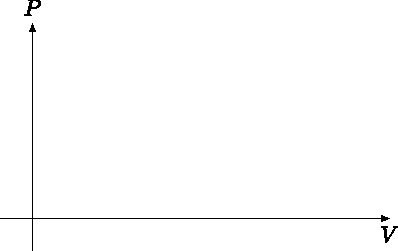
\includegraphics[width=\linewidth, valign=t]{cycle_lenoir-plain}
			}{
				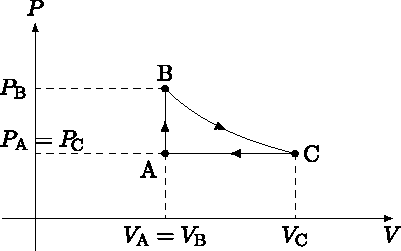
\includegraphics[width=\linewidth, valign=t]{cycle_lenoir}
			}
			\captionof{figure}{Cycle de \textsc{Lenoir}.}
		\end{center}
	\end{isd}
	\begin{enumerate}[label=\sqenumi]
		\item Tracer ce cycle dans le diagramme de \textsc{Watt}. Déterminer la
		      nature du cycle (moteur ou récepteur).
		\item Calculer la pression, le volume et la température pour chacun des
		      états $A$, $B$ et $C$.
		\item Calculer les travaux associés à chaque transformation puis celui du
		      cycle. Vérifier sa nature.
	\end{enumerate}
	\tcblower
	\begin{enumerate}[label=\sqenumi]
		\item Voir la figure ci-dessus. Pour la nature, on voit que
		      \psw{le cycle s'effectue en \textbf{sens horaire}, donc $W_{p,\rm
						      cycle} < 0$ donc \textbf{moteur}}.
		\item
		      \begin{enumerate}[label=\clalphi]
			      \item On a déjà $P_A$ et $V_A$, on cherche $T_A$~:
			            \psw{%
				            \[
					            \boxed{T_A = \frac{P_AV_A}{nR}}
					            \Ra
					            \xul{T_A = \SI{337}{K}}
					            \qav
					            \left\{
					            \begin{array}{rcl}
						            P_A & = & \SI{2e5}{Pa}
						            \\
						            V_A & = & \SI{1.4e-2}{m^3}
						            \\
						            n   & = & \SI{1}{mol}
						            \\
						            R   & = & \SI{8.314}{J.K^{-1}.mol^{-1}}
					            \end{array}
					            \right.
				            \]
			            }%
			      \item On connaît $P_B$ et transformation isochore donc
			            $\setlength{\fboxsep}{3mm}\boxed{\psw{V_B = V_A}}$, on cherche $T_B$~:
			            \psw{%
				            \[
					            \boxed{T_B = \frac{P_BV_B}{nR}}
					            \Ra
					            \xul{T_B = \SI{674}{K}}
				            \]
			            }%
			      \item On connaît $V_C = 2V_B$ et transformation isotherme donc
			            $\setlength{\fboxsep}{3mm}\boxed{\psw{T_C = \SI{674}{K}}}$, on cherche
			            $P_C$~:
			            \psw{%
				            \[
					            \boxed{P_C = \frac{nRT_C}{V_C}}
					            \Ra
					            \xul{P_C = \SI{2e5}{Pa}}
				            \]
			            }%
		      \end{enumerate}
		\item On a déjà démontré les formules utiles, mais \textbf{il faudrait
			      les redémontrer} pour ne pas se tromper de signe.
		      \begin{itemize}
			      \item
			            \leftcenters{%
				            \psw{%
					            AB~: transformation isochore, donc
				            }%
			            }{%
				            \psw{%
					            $\boxed{W_{p,\rm AB} = 0}$
				            }%
			            }%
			      \item
			            \leftcenters{%
				            \psw{%
					            BC~: isoT et Q.S. donc
				            }%
			            }{%
				            \psw{%
					            $
						            % W_{p,\rm BC} = nRT_B \ln (\frac{V_B}{V_C})
						            %       \Lra
						            \boxed{W_{p,\rm BC} = -nRT_B \ln 2}
						            \Ra
						            \xul{W_{p,BC} = \SI{-3.88}{kJ}}
					            $
				            }%
			            }%
			      \item
			            \leftcenters{%
				            \psw{%
					            CA~: isobare, donc
				            }%
			            }{%
				            \psw{%
					            $
						            % W_{p,\rm CA} = P_C (V_C - V_A)
						            %       \Lra
						            \boxed{W_{p,\rm CA} = 2P_AV_A}
						            \Ra
						            \xul{W_{p,CA}= \SI{2.8}{kJ}}
					            $
				            }%
			            }%
			      \item
			            \leftcenters{%
				            \psw{%
					            Cycle~:
				            }%
			            }{%
				            \psw{%
					            $\DS
						            W_{p,\rm cycle} = \sum_i W_i = W_{AB} + W_{BC} + W_{CA} =
						            % + 2P_AV_A - nRT_B \ln 2
						            \SI{-1.08}{kJ}
					            $
				            }%
			            }%
			            \smallbreak
			            \psw{%
				            Il reçoit bien un travail \textbf{négatif}, c'est donc
				            un cycle \textbf{moteur} comme prédit.
			            }%
		      \end{itemize}
	\end{enumerate}
\end{tcb*}

\section{Transfert thermique}
\label{sec:transtherm}
\subsection{Définition}
\begin{tcb*}(defi){Transfert thermique}
	Un système thermodynamique peut recevoir de l'énergie sans l'intercention
	d'une action mécanique mesurable à l'échelle macroscopique. Ce transfert
	d'\textbf{énergie microscopique}, complémentaire du travail mécanique s'appelle
	\textbf{transfert thermique}, noté $Q$.
\end{tcb*}

\begin{tcb}(rema)<lftt>{$Q$}
	Comme le travail, c'est une \textbf{énergie}, et comme le travail, il
	\textbf{dépend du chemin suivi}.
\end{tcb}
\subsection{Types de transferts thermiques}
\begin{tcb}(defi){Convection, conduction et rayonnement}
	Les transferts thermiques peuvent se faire selon trop modes de transport~:
	\begin{itemize}
		\bitem{Convection}~: \psw{dans les \textbf{fluides}, les masses en
			\textbf{mouvement} transportent leur énergie interne et permettent les
			échanges de chaleur}
		\bitem{Conduction}~: \psw{dans les \textbf{solides}, la chaleur se propage
			\textbf{sans déplacement} mais de prochee en proche, des zones chaudes vers
			les zones froides}
		\bitem{Rayonnement}~: \psw{transfert \textbf{par les ondes}, sans besoin de
			matière~: l'onde transporte son énergie qui peut être absorbée et
			transformée en agitation thermique}
	\end{itemize}
\end{tcb}

\begin{tcb}(exem)<lftt>{Modes de transfert thermique}
	\begin{isd}[righthand ratio=.4]
		On observe ces trois phénomènes en même temps en faisant bouillir de l'eau sur
		une gazinière~:
		\begin{itemize}
			\bitem{Convection}~: \psw{l'eau qui bout transporte la chaleur du fond vers
				le haut}
			\bitem{Conduction}~: \psw{le manche de la casserole devient de plus en plus
				chaud au fur et à mesure}
			\bitem{Rayonnement}~: \psw{le feu envoie directement de la chaleur sous
				forme d'onde électromagnétique}
		\end{itemize}
		\tcblower
		\begin{center}
			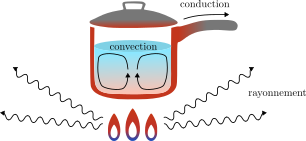
\includegraphics[width=\linewidth]{transtherm_casserole}
		\end{center}
	\end{isd}
	D'autres exemples~:
	\smallbreak
	\noindent
	\begin{minipage}[t]{.31\linewidth}
		\tcbsubtitle{\fatbox{\textbf{Convection}}}
		\begin{itemize}
			\item \psw{Courant d'air froid}
			\item \psw{De la crème dans la soupe}
			\item \psw{Four à convection~!}
		\end{itemize}
	\end{minipage}
	\hfill
	\begin{minipage}[t]{.31\linewidth}
		\tcbsubtitle{\fatbox{\textbf{Conduction}}}
		\begin{itemize}
			\item \psw{Transfert par les vitres}
			\item \psw{Toucher du métal\ftn{Dû à leur grande conductivité thermique.}}
			\item \psw{Tisonnier dans le feu}
		\end{itemize}
	\end{minipage}
	\hspace*{\fill}
	\begin{minipage}[t]{.31\linewidth}
		\tcbsubtitle{\fatbox{\textbf{Rayonne\mnt}}}
		\begin{itemize}
			\item \psw{Soleil}
			\item \psw{N'importe quel corps chaud}
			\item \psw{Applica$^\circ$~: couvertures de survie}
		\end{itemize}
	\end{minipage}
\end{tcb}

\subsection{Cas particuliers}
\subsubsection{Thermostat}
\begin{tcb*}(defi){Thermostat}
	Un \textbf{thermostat} est un système thermodynamique dont la
	\textbf{température reste constante}, \xul{même s'il échange de l'énergie}~:
	\psw{%
		\[
			\boxed{T\ind{thermostat} = \cte}
		\]
	}%
	\vspace{-15pt}
\end{tcb*}

\begin{tcb}(inte){Thermostat}
	On peut voir un thermostat comme un très grand volume, de capacité thermique
	infinie~:
	\psw{%
		\[
			\boxed{C_{V}\sup{thermostat} = +\infty}
		\]
	}%
	Ainsi, il faut lui apporter une énergie infinie pour élever sa température
	d'un degré~: il peut transmettre de la chaleur mais on ne peut pas changer sa
	température~!
\end{tcb}

\begin{tcb}(exem)<lftt>{Thermostats}
	\begin{itemize}
		\item \psw{L'atmosphère sur une courte durée}
		\item \psw{Thermostat d'un four}
		\item \psw{Un bain-marie}
	\end{itemize}
\end{tcb}

\subsubsection{Transformations adiabatiques}
\begin{tcb*}(defi){Transformation adiabatique}
	Une transformation est dite \textbf{adiabatique} s'il n'y a \textbf{pas
		de transfert thermique}~:
	\psw{%
		\[
			\boxed{Q = 0}
		\]
	}%
	Dans ce cas, le système est dit \xul{\psw{\textbf{calorifugé}}}
\end{tcb*}

\begin{tcb}(exem)<lftt>{Transformation adiabatique}
	C'est le principe des bouteilles thermos et et calorimètres. Ils fonctionnent
	grâce à~:
	\begin{itemize}
		\item \psw{Une pellicule de vide entre le vase intérieur et extérieur pour
			      limiter la convection et la conduction}
		\item \psw{Une surface réfléchissante limitant les transferts par
			      rayonnement}
	\end{itemize}
\end{tcb}

\begin{tcb}(impl)<lftt>{Transformation adiabatique}
	Dans le cas d'une transformation adiabatique, la température du système dans
	l'état final n'est \textbf{pas déterminée par une condition d'équilibre}
	thermique, puisque le système n'est en contact thermique avec aucun autre
	système.
\end{tcb}

L'efficacité d'un tel dispositif est limitée dans le temps et le système finit
toujours par être en équilibre thermique avec l'extérieur. Le rôle de
l'isolation thermique est d'augmenter fortement le temps caractéristique
d'établissement de l'équilibre thermique. Celui-ci peut facilement devenir
très long.

\subsection{Bien comprendre les transferts}
\subsubsection{Retour sur mono- et isotherme}

\begin{tcb*}(coro){Reformulation de monotherme}
	Une transformation est \textbf{monotherme} si le système n'échange de la
	chaleur qu'\textbf{avec un seul thermostat}.
\end{tcb*}

Pour qu'une transformation soit \textbf{isotherme} il faut que la
\textbf{température} du système ne \textbf{varie pas}. Or dans la plupart des
cas\ftn{L'exception est l'équilibre diphasé, sujet d'un prochain chapitre.}, tout
apport d'énergie au système tend à faire varier sa température.
\bigbreak
La réalisation d'une transformation isotherme nécessite donc un
\textbf{contrôle} de la température que l'on obtient en mettant le système en
contact avec un \textbf{thermostat}. Il faut que les échanges thermiques entre
le système et le thermostat soient faciles. Ceux-ci doivent donc être séparés
par une paroi diathermane~:
\begin{tcb}(defi)<lftt>{Diathermane}
	Est \textbf{diathermane} une paroi laissant \textbf{passer la chaleur}.
\end{tcb}
De plus, l'évolution du système doit être \textbf{suffisamment lente} pour que
les échanges thermiques aient le temps de s'établir et assurent le maintien de
la température $T$ du système à la même valeur que la température $T_0$ du
thermostat.

\begin{tcb*}(ror){Transferts thermiques particuliers}
	\begin{itemize}
		\item \psw{Les cas limites adiabatique et isotherme sont des \textbf{cas
				      limites}, approximations de la réalité.}
		\item \psw{Une \textbf{transformation lente} au contact d'un
			      \textbf{thermostat} est en général \textbf{isotherme}, donc en
			      équilibre thermique à tout instant.}
		\item \psw{Les équilibres mécaniques sont en général \textbf{rapides} devant
			      les équilibres thermiques~; ainsi \textbf{une transformation rapide
				      peut être considérée comme adiabatique}, comme les transferts n'ont
			      pas le temps de se faire}
	\end{itemize}
\end{tcb*}

\subsubsection{Adiabatique ou isotherme~?}

\begin{tcb*}(impo){Adiabatique vs.\ isotherme}
	Il est commun de confondre adiabatique et isotherme. Pourtant, les
	transformations isotherme et adiabatique sont deux transformations idéales aux
	caractères \textbf{diamétralement opposés}~:
	\begin{itemize}
		\bitem{Isotherme} veut dire que la température est définie et constante à
		tout instant de la transformation, \textbf{grâce} aux échanges thermiques
		avec un thermostat~;
		\bitem{Adiabatique} suppose une \textbf{absence} d'échanges thermiques.
	\end{itemize}
\end{tcb*}
Une transformation réelle pourra se rapprocher de l'une ou l'autre des ces deux
transformations limites, et il importe de savoir choisir la bonne modélisation.

\begin{tcb}[breakable](exem)<lftt>{Adiabatique vs.\ isotherme}
	Un gaz est contenu dans un récipient fermé par un piston de surface $S$, sur
	lequel on exerce une force $\Ff$ variable, avec $\Ff_i$ et $\Ff_f$ dans l'état
	initial et final. On impose, par la condition d'équilibre mécanique du piston,
	une pression $P = \frac{F}{S}$ au gaz.
	\tcbsubtitle{\fatbox{\textbf{Isotherme}}}
	\begin{isd}
		Le récipient a des parois fines, \textbf{diathermanes} dans un milieu
		extérieur \textbf{thermostaté} à $T\ind{ext} = T_0$. On augmente
		\textbf{lentement} la force $\Ff$, provoquant une descente progressive du
		pistant et laissant le gaz s'\textbf{équilibrer thermiquement} à chaque
		instant~: c'est une \textbf{compression isotherme}.
		\tcblower
		\begin{center}
			\sswitch{
				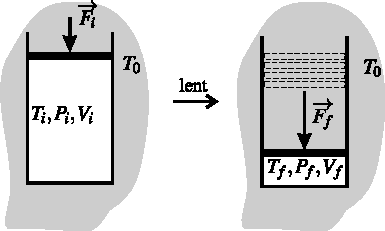
\includegraphics[width=\linewidth, draft=true]{exem_isoT}
			}{
				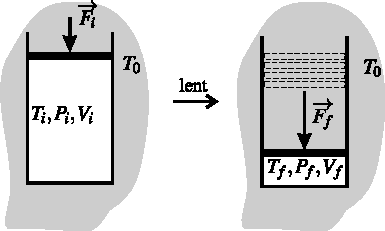
\includegraphics[width=\linewidth]{exem_isoT}
			}
		\end{center}
	\end{isd}
	On obtient alors tous les paramètres d'état du gaz dans l'état final~:
	\psw{%
		\[
			P_f = \frac{F_f}{S}
			\qet
			T_f = T_0
			\qet
			V_f = V_i\frac{P_i}{P_f}\frac{T_0}{T_i}.
		\]
	}%
	\tcbsubtitle{\fatbox{\textbf{Adiabatique}}}
	\begin{isd}
		Le récipient a des \textbf{parois épaisses}. On augmente \textbf{rapidement}
		la force $\Ff$, l'échange \textbf{thermique} n'a \textbf{pas le temps} de se
		faire~: c'est une \textbf{compression adiabatique}.
		\tcblower
		\begin{center}
			\sswitch{
				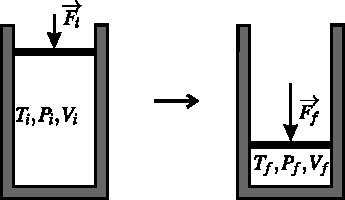
\includegraphics[width=\linewidth, draft=true]{exem_adia}
			}{
				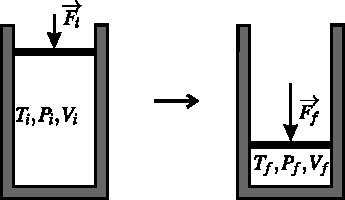
\includegraphics[width=\linewidth]{exem_adia}
			}
		\end{center}
	\end{isd}
	Dans ce cas, l'équation d'état ne suffit pas pour trouver l'état final, on n'a
	pas de renseignement sur $T_f$.
\end{tcb}

\begin{tcn}*(coro)<ctb>"trans"{Transition}
	Dans l'exemple précédent, on peut cependant supposer qu'elle soit à la
	fois \textit{adiabatique} et \textit{mécaniquement réversible}, c'est-à-dire
	suffisamment rapide pour qu'il n'y ait pas de transfert thermique, mais
	suffisamment lente pour qu'il y ait équilibre mécanique à chaque instant. On
	pourra dans ce cas utiliser une autre équation d'état, la \textsc{loi de
		\textsc{Laplace}}.
\end{tcn}

\subsection{Loi de \textsc{Laplace}}
\begin{tcb*}(prop){Loi de \textsc{Laplace}}
	Pour une transformation \textbf{adiabatique} et \textbf{mécaniquement
		réversible} d'un \textbf{gaz parfait}, les paramètres d'état sont reliés par
	les relations suivantes~:
	\psw{%
	\[
		PV^{\gamma} = \cte
		\qqet
		P^{1-\gamma}T^{\gamma} = \cte
		\qqet
		TV^{\gamma-1} = \cte
	\]
	}%
	où $\gamma > 1$ est le coefficient adiabatique du fluide.
\end{tcb*}
\begin{tcb}(rema)<lftt>{}
	\begin{itemize}
		\item Elle sera démontrée dans un chapitre ultérieur. On introduit $\gamma$ dans le
		      chapitre suivant.
		\item Il ne suffit d'en apprendre qu'une seule, par exemple $PV^{\gamma} =
			      \cte$ pour retrouver les autres~:
		      \begin{tasks}[label=\btrg](2)
			      \task Pour $TV^{\gamma-1}$~:
			      \psw{%
				      \begin{gather*}
					      PV^{\gamma} = \cte
					      \qet
					      P = \frac{nRT}{V}
					      \\\Ra
					      \frac{nRT}{V}V^{\gamma} = \cte
					      \\\Lra
					      \boxed{TV^{\gamma-1} = \cte}
				      \end{gather*}
			      }%
			      \vspace{-15pt}
			      \task Pour $P^{1-\gamma}T^{\gamma}$~:
			      \psw{%
				      \begin{gather*}
					      PV^{\gamma} = \cte
					      \qet
					      V = \frac{nRT}{P}
					      \\\Ra
					      P \left( \frac{nRT}{P} \right)^{\gamma} = \cte
					      \\\Lra
					      \boxed{P^{1-\gamma}T^{\gamma} = \cte}
				      \end{gather*}
			      }%
			      \vspace{-15pt}
		      \end{tasks}
	\end{itemize}
	\vspace{-15pt}
\end{tcb}

\begin{tcb}(appl)<lftt>{Loi de \textsc{Laplace}}
	On prend $V_i = \SI{20}{L}$ de gaz à $T_i = \SI{293}{K}$ et sous $P_i =
		\SI{1}{bar}$. On comprime ce gaz de façon adiabatique et mécaniquement
	réversible jusqu'au volume $V_f = \SI{10}{L}$. On donne $\gamma = \num{1.4}$~:
	calculer la pression et la température.
	\tcblower
	\begin{isd}
		\begin{itemize}
			\item Pression~:
			      \psw{%
				      \begin{gather*}
					      P_iV_i^{\gamma} = P_fV_f^{\gamma}
					      \\\Lra
					      \boxed{P_f = P_i \frac{V_i^{\gamma}}{V_f^{\gamma}}}
					      \Ra
					      \xul{P_f = \SI{2.64}{bars}}
				      \end{gather*}
			      }%
		\end{itemize}
		\tcblower
		\begin{itemize}
			\item Température~:
			      \psw{%
				      \begin{gather*}
					      T_iV_i^{\gamma-1} = T_fV_f^{\gamma-1}
					      \\\Lra
					      \boxed{T_f = T_i \frac{V_i^{\gamma-1}}{V_f^{\gamma-1}}}
					      \Ra
					      \xul{T_f = \SI{387}{K}}
				      \end{gather*}
			      }%
		\end{itemize}
	\end{isd}
\end{tcb}

\begin{tcb*}(impo){Loi de \textsc{Laplace}}
	Il est nécessaire de \textbf{connaître} et \textbf{citer} les
	conditions d'applications~:
	\begin{tasks}[label=\bdmd]
		\task \psw{Adiabatique $Q=0$~;}
		\task \psw{Mécaniquement réversible~: $P = P\ind{ext}$~;}
		\task \psw{Gaz parfait.}
	\end{tasks}
\end{tcb*}

\begin{tcb*}[list
	entry={\hspace*{-20pt}\protect\rcheck~
	Adia.\ vs.\ isoT.\ en $(P,V)$}]
	(ror){Adiabatique et isotherme en $(P,V)$}
	Il faut savoir distinguer une isotherme d'une adiabatique en diagramme
	de \textsc{Watt} ou \textsc{Clapeyron} (quand la transformation est
	mécaniquement réversible)~:
	\noindent
	\begin{minipage}[c]{.65\linewidth}
		\begin{itemize}
			\bitem{Isotherme} $\Ra P \propto 1/V$~;
			\bitem{Adiabatique} $\Ra P \propto 1/V^{\gamma}$ donc \textbf{plus raide}
		\end{itemize}
		On peut aussi les retrouver par l'intuition~:
		\begin{itemize}
			\item Compression isotherme $\Ra V \searrow$ et $T=\cte$ donc \xul{\psw{$P
						      \nearrow$}}~;
			\item Compression adiabatique $\Ra V \searrow$, mais $T \nearrow$ donc
			      \xul{\psw{$P \nearrow\nearrow$}}.
		\end{itemize}
	\end{minipage}
	\hfill
	\begin{minipage}[c]{.33\linewidth}
		\begin{center}
			\sswitch{
				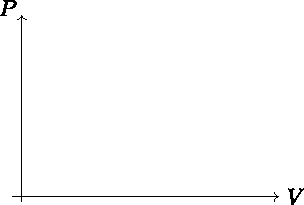
\includegraphics[width=\linewidth]{iso_vs_adia-plain}
			}{
				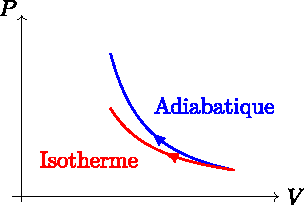
\includegraphics[width=\linewidth]{iso_vs_adia}
			}
			\vspace{-15pt}
			\captionof{figure}{IsoT.\ vs.\ adiabatique en $(P,V)$}
		\end{center}
	\end{minipage}
\end{tcb*}

\end{document}
